% !TEX root = ../../main.tex
% !TeX spellcheck = de_DE

\chapter{Diskussion}
Ziel der Studienarbeit ist es, möglichst gute Architekturen inklusive Hyperparameterkombinationen zu finden.
Dafür werden in diesem Kapitel die Trainingsergebnisse des Dense-, und DC-GANs verglichen und interpretiert.

\section{Zusammenfassung der Ergebnisse}
Die besten Ergebnisse erzielt das Dense GAN, das ausschließlich aus Dense Layern besteht.
Es ist in der Lage erkennbare Figuren zu erzeugen, die vom vorgegebenen Label abhängig sind.
Dabei ist anzumerken, dass der beste FID-Wert nicht mit den subjektiv besten Ergebnissen übereinstimmt.
\newline

Nach einem zusätzlichen Training einer vielversprechenden Architektur sind die Figuren auch deutlich klarer abgebildet.
Allerdings hat das Dense GAN immer starke Schwierigkeiten mit Rauschen.
So sind zum einen immer Pixelfragmente im Bild zu erkennen, zum anderen besitzen die Formen keine klaren Ränder.

\begin{figure}[H]
	\centering
	\subfloat[][]{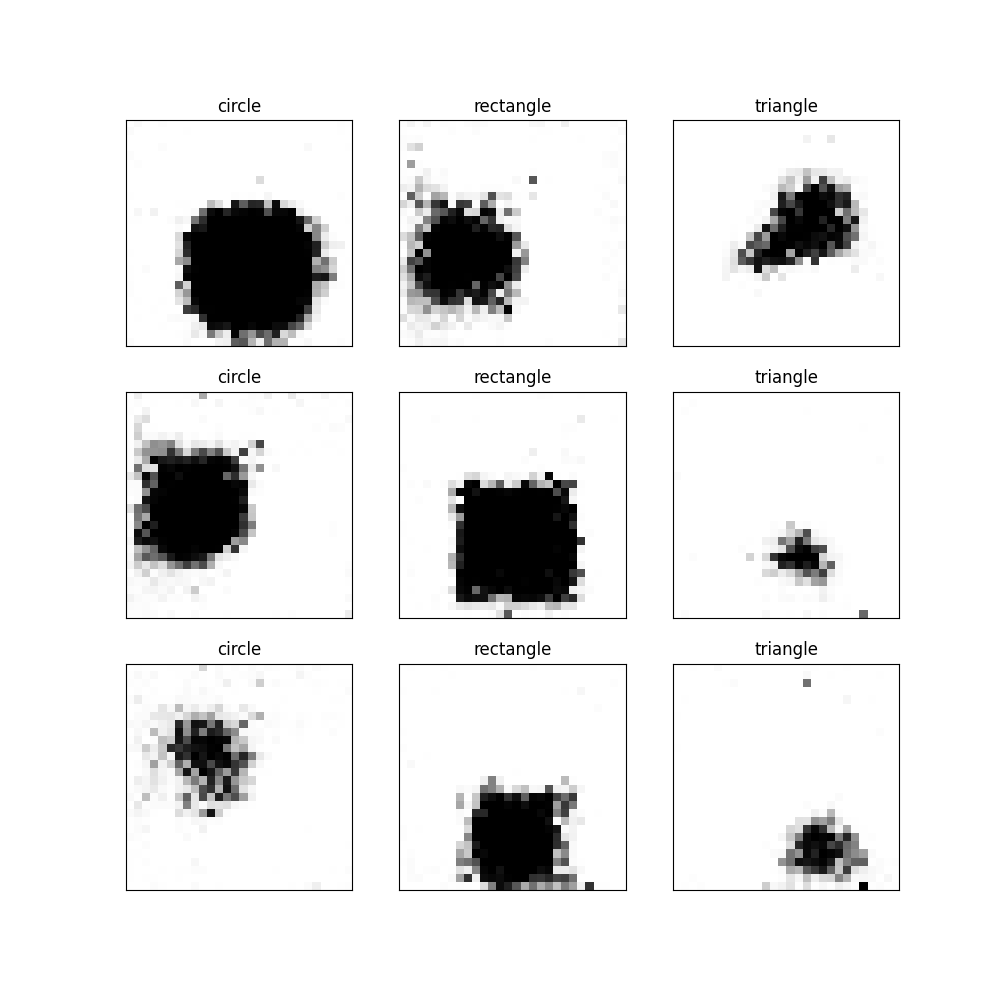
\includegraphics[width=0.45\linewidth]{kapitel/5_ergebnisse/densegan/good_example.png}}
	\qquad
	\subfloat[][]{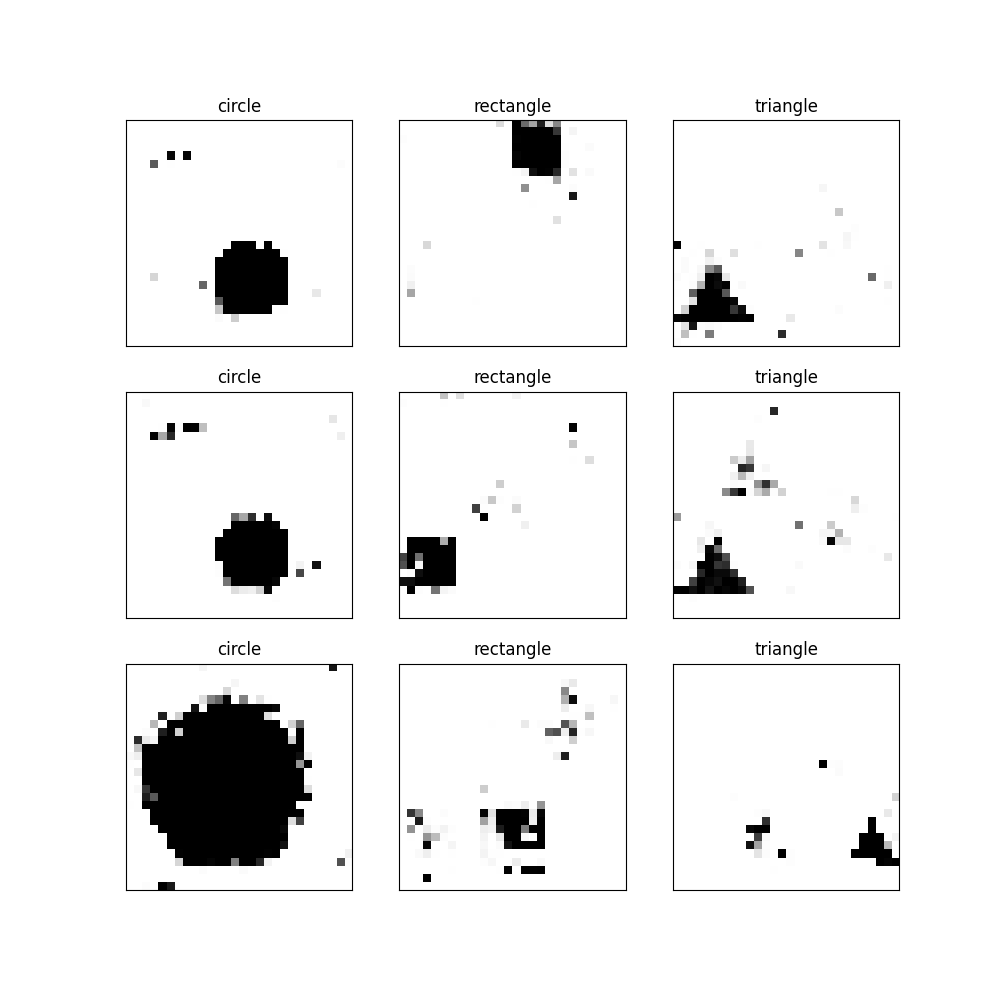
\includegraphics[height=0.35\textheight]{kapitel/5_ergebnisse/densegan/good_example_long.png}}
	\label{ergebnis:densegan-zusammenfassung}
	\caption[]{\textbf{a)} die subjektiv besten Ergebnisse nach regulärem Training; \textbf{b)} Ergebnisse nach zusätzlichem Training; \\auf beiden Bildern lässt sich starkes Rauschen erkennen}
\end{figure}

Probleme mit Rauschen existieren beim DC-GAN fast gar nicht, die Figuren sind alle sehr klar abgebildet.
Es existieren auch vergleichsweise wenig zusätzliche Pixelfragmente und wenn gibt es zumindest ähnliche Formmerkmale bei beiden Fragmenten, wie in \cref{ergebnis:dcgan-fid-zusammenfassung} zu sehen.
\newline

Allerdings ist die Bildqualität der DC-GAN-Bilder deutlich schlechter.
Oftmals wird eine Figur erzeugt, die Merkmale mehrere Kategorien besitzt.
Dadurch lässt sich nicht immer eindeutig eine Figur zuordnen.

\begin{figure}[H]
	\centering
	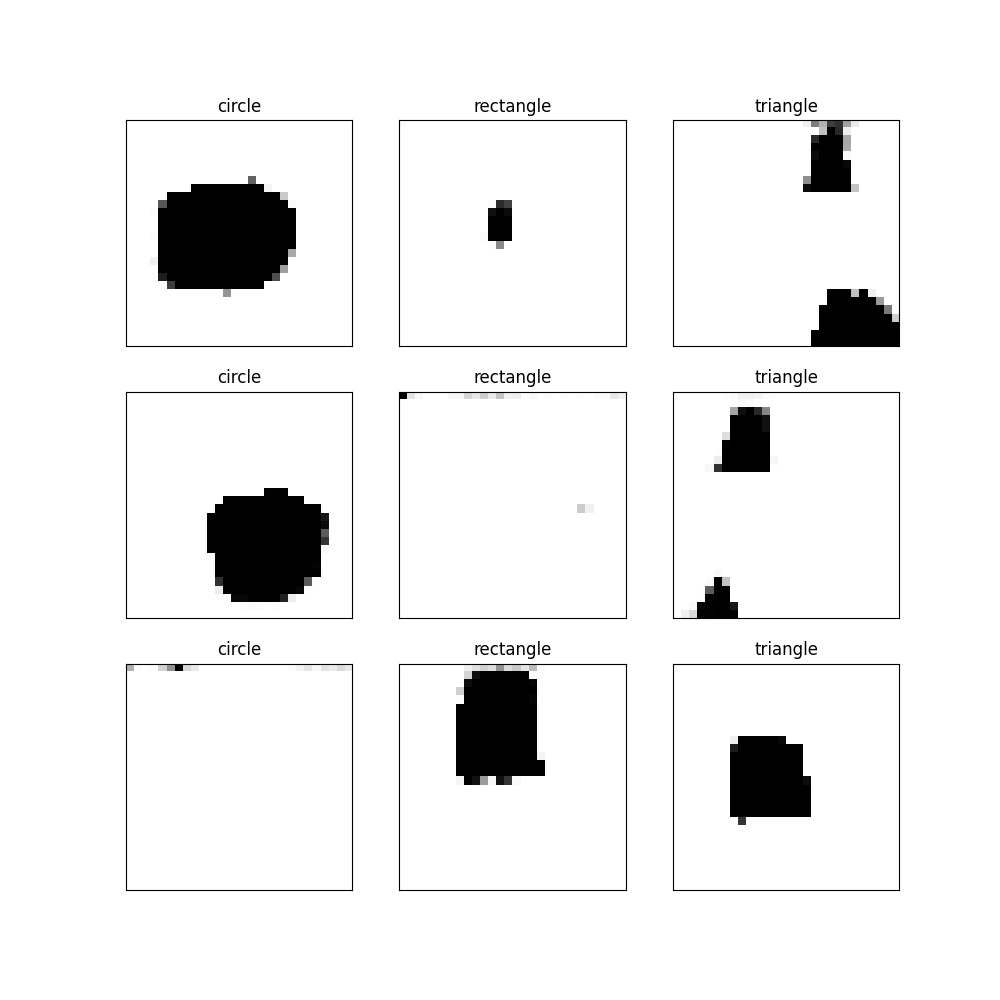
\includegraphics[width=0.45\linewidth]{kapitel/5_ergebnisse/dcgan/fid_circle.png}
	\label{ergebnis:dcgan-fid-zusammenfassung}
	\caption[]{\textbf{Oben Links:} ein Kreis mit einer geraden Kante; \textbf{Mitte Rechts:} zwei Pixelfragmente mit den schrägen Kanten eines Dreiecks}
\end{figure}


\section{Interpretation der Ergebnisse}
Beide Architekturen erzeugen Bilder, die Gemeinsamkeiten mit den Trainingsdaten aufzeigen.
Unterschiede gibt es vor allem beim Rauschen und der Unterscheidbarkeit der Figuren.

\subsubsection{Rauschen}
Das Dense-GAN hat größere Probleme mit Rauschen.
Das lässt sich auf die Layerarchitektur zurück führen, da im Gegensatz zu Convolutional Layern die Pixel separater betrachtet werden.
So erzeugt das DC-GAN zusätzliche Figuren als Fragmente, während beim Dense-GAN einzelne Pixel falsch eingefärbt werden.

\subsubsection{Unterscheidbarkeit der Formen}
Beide GANs neigen zur Vermischung von Eigenschaften unterschiedlicher Figuren, zum Beispiel ein Kreis mit einer geraden Kante.
Durch das prototypische Zusatztraining beim Dense GAN nehmen die Ähnlichkeiten zwischen den Figuren aber ab.

\section{Beschränkung der Forschung}
Für das Training und somit auch die Ergebnisse war insbesondere die verfügbare Hardware ein große Beschränkung.
Mit besserer Hardware hätten unter anderem mehr Hyperparameterkombinationen ausprobiert oder ein deutlich längeres Training durchgeführt werden.
\newline

Die Trainingsdaten besitzen auch kein Bildrauschen oder ähnliche Verfälschungen.
Das würde das Training zusätzlich erschweren, aber gleichzeitig die entstehenden Netze robuster machen.

\section{Ausblick}
Für zukünftige Forschung lassen sich insbesondere die Trainingsdaten weiter anpassen und die angesprochene Verfälschung der Bilder einbauen.
Außerdem besteht die Möglichkeit die Figuren auf den Figuren alle zu zentrieren und skalieren, sodass sie das Bild komplett ausfüllen.
Das ist insofern interessant, als dass das mit Algorithmen möglich ist, es wird kein Training benötigt.
Folglich könnten die Daten in der Vorverarbeitung (Preprocessing) dementsprechend angepasst werden.
Dann könnte ein Vergleich zwischen vorverarbeiteten und unvorverarbeiteten Daten gezogen werden.
\newline

Des Weiteren können die vorgestellten Architekturen weiter trainiert werden.
Wie durch das Dense GAN gezeigt, können die Ergebnisse mit mehr Training noch weiter verbessert werden.
Zusätzlich könnten bei viel Hardware Kapazitäten auch die Hyperparameter noch einmal mit dem Genetic Algorithm optimiert werden.
